
\section{Regular Feature}

\begin{frame}
  \frametitle{引用别人的话}
  \begin{quotation}
    "There is nothing new to be discovered in physics now. All that remains is 
    more and more precise measurements"   \\
    \rightline{$\cdots$ Lord Kelvin (1900)\hspace{3em}}
\end{quotation}  
\end{frame}

\begin{frame}
  \frametitle{公式加框 boxed}
  \begin{equation}
    \boxed{\rho(\nu, T) d \nu=\frac{8 \pi}{c^{3}} \frac{h \nu^{3}}{e^{h \nu / K T}-1} d \nu}
  \end{equation}
\end{frame}

\begin{frame}
  \frametitle{内容加框boxedminipage}
  \begin{boxedminipage}{0.9\linewidth}
   % \vspace{-15pt}
    \[\begin{aligned}
    & \text{若}X_i\sim N(\mu_i,\sigma_i^2)\, i=1,2,\cdots,\text{且它们相互独立,则其线性组合:}\\
    & c_0+c_1X_1+c_2X_2+\cdots+c_nX_n\sim N(\mu,\sigma^2)\\
    & \text{其中}c_1,c_2,\cdots,c_n \text{是不全为0的常数,两个参数为:}\\
    & \mu=c_0+c_1\mu_1+\cdots+c_n\mu_n,\qquad \sigma^2=c_1^2\sigma_1^2+c_2^2\sigma_2^2+\cdots+c_n^2\sigma_n^2
    \end{aligned}\]
    \vspace{2pt}
    \end{boxedminipage}
\end{frame}

\begin{frame}{Font feature test}
  \begin{itemize}
    \item Regular
    \item \textit{Italic}
    \item \textsc{Small Caps}
    \item \textbf{Bold}
    \item \textbf{\textit{Bold Italic}}
    \item \textbf{\textsc{Bold Small Caps}}
    \item \texttt{Monospace}
    \item \texttt{\textit{Monospace Italic}}
    \item \texttt{\textbf{Monospace Bold}}
    \item \texttt{\textbf{\textit{Monospace Bold Italic}}}
  \end{itemize}
\end{frame}

\begin{frame}{Columns and Lists}
  \begin{columns}[T,onlytextwidth]
    \column{0.33\textwidth}
      Items
      \begin{itemize}
        \item Milk \item Eggs \item Potatoes
      \end{itemize}

    \column{0.33\textwidth}
      Enumerations
      \begin{enumerate}
        \item First, \item Second and \item Last.
      \end{enumerate}

    \column{0.33\textwidth}
      Descriptions
      \begin{description}
        \item[PowerPoint] Meeh. \item[Beamer] Yeeeha.
      \end{description}
  \end{columns}
\end{frame}

\begin{frame}{Tables}
  \begin{table}
    \caption{Largest cities in the world (source: Wikipedia)}
    \begin{tabular}{@{} lr @{}}
      \toprule
      City & Population\\
      \midrule
      Mexico City & 20,116,842\\
      Shanghai & 19,210,000\\
      Peking & 15,796,450\\
      Istanbul & 14,160,467\\
      \bottomrule
    \end{tabular}
  \end{table}
\end{frame}


\begin{frame}{Math}
  \begin{equation*}
    e = \lim_{n\to \infty} \left(1 + \frac{1}{n} \right)^n
  \end{equation*}
\end{frame}

\begin{frame}{Blocks}
  Three different block environments are pre-defined and may be styled with an
  optional background color.

  \begin{columns}[T,onlytextwidth]
    \column{0.48\textwidth}
      \begin{block}{Default}
        Block content.
      \end{block}

      \begin{alertblock}{Alert}
        Block content.
      \end{alertblock}

      \begin{exampleblock}{Example}
        Block content.
      \end{exampleblock}

    \column{0.48\textwidth}

      %\metroset{block=fill}

      \begin{block}{Default}
        Block content.
      \end{block}

      \begin{alertblock}{Alert}
        Block content.
      \end{alertblock}

      \begin{exampleblock}{Example}
        Block content.
      \end{exampleblock}

  \end{columns}
\end{frame}

\section{tikz}


\begin{frame}{tikz for Figures}
  \begin{figure}
    \newcounter{density}
    \setcounter{density}{20}
    \begin{tikzpicture}
      \def\couleur{alerted text.fg}
      \path[coordinate] (0,0)  coordinate(A)
                  ++( 90:5cm) coordinate(B)
                  ++(0:5cm) coordinate(C)
                  ++(-90:5cm) coordinate(D);
      \draw[fill=\couleur!\thedensity] (A) -- (B) -- (C) --(D) -- cycle;
      \foreach \x in {1,...,40}{%
          \pgfmathsetcounter{density}{\thedensity+20}
          \setcounter{density}{\thedensity}
          \path[coordinate] coordinate(X) at (A){};
          \path[coordinate] (A) -- (B) coordinate[pos=.10](A)
                              -- (C) coordinate[pos=.10](B)
                              -- (D) coordinate[pos=.10](C)
                              -- (X) coordinate[pos=.10](D);
          \draw[fill=\couleur!\thedensity] (A)--(B)--(C)-- (D) -- cycle;
      }
    \end{tikzpicture}
    \caption{Rotated square from
    \href{http://www.texample.net/tikz/examples/rotated-polygons/}{texample.net}.}
  \end{figure}
\end{frame}

\begin{frame}{Line plots}
  \begin{figure}
    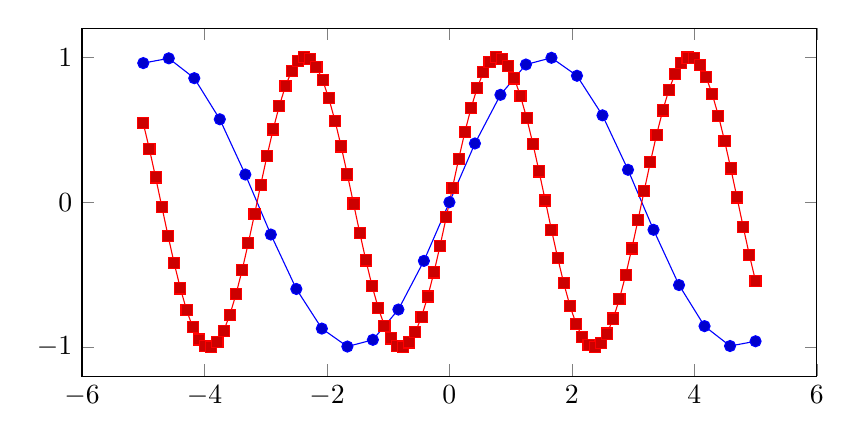
\begin{tikzpicture}
      \begin{axis}[
        width=0.9\textwidth,
        height=6cm,
      ]

        \addplot {sin(deg(x))};
        \addplot+[samples=100] {sin(deg(2*x))};

      \end{axis}
    \end{tikzpicture}
  \end{figure}
\end{frame}


\begin{frame}{3D plots}
\begin{figure}
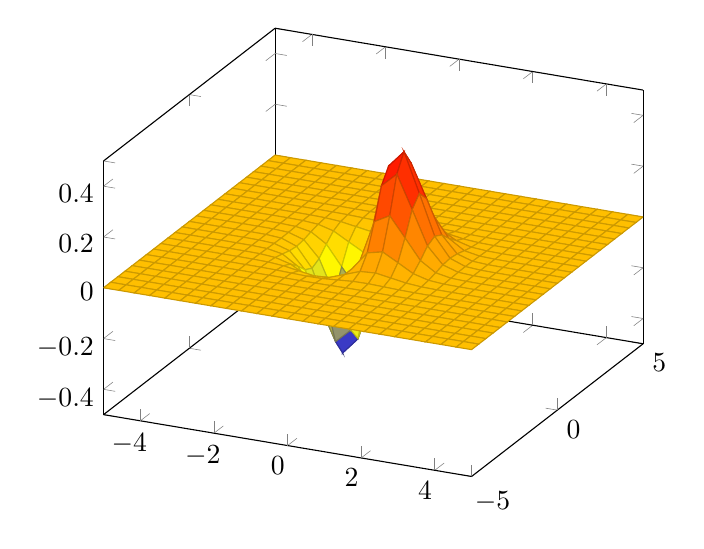
\begin{tikzpicture}
  \begin{axis}
  \addplot3[
      surf,
  ]
  {exp(-x^2-y^2)*x};
  \end{axis}
  \end{tikzpicture}
\end{figure}
\end{frame}
%%%%%%%%%%%%%%%%%%%%%%%%%%%%%%%%%%%%%%%%%%%%%%%%%

\begin{frame}
  \frametitle{}
  \tikzboxtitle{Fermat's Last Theorem}
  \centering
  \tikzbox[0.5]{
       Fermat's Last Theorem states that
       \[ x^n + y^n = z^n\]
       has no non-zero integer solutions for $x$, $y$ and $z$ when $n > 2$.
  }
\end{frame}

\section{区块环境}

\begin{frame}
\frametitle{1.block}
	\begin{block}{勾X定理:}
		直角三角形的斜边的平方等于两直角边的平方和。
		可以用符号语言表述为:设直角三角形ABC,其中$\angle C=90^\circ $则有
		\begin{equation}
			AB^2=BC^2+AC^2 \int
		\end{equation}
	\end{block}
	\begin{block}{Remark}
		Sample text
	\end{block}
\end{frame}

\begin{frame}
    \frametitle{2.alertblock}
	\begin{alertblock}{Important theorem}
		Sample text in red box
	\end{alertblock}
\end{frame}

\begin{frame}
    \frametitle{3.exampleblock}
	\begin{exampleblock} {Exampleblock}
		Sample text in green box. The title of the block is 'Examples'.
	\end{exampleblock}
    \begin{exampleblock} {例1:}
		Sample text in green box. The title of the block is 'Examples'.
	\end{exampleblock}
\end{frame}

\begin{frame}
    \frametitle{4.examples}
	\begin{examples}
		Sample text in green box. The title of the block is 'Examples'.
	\end{examples}
  \begin{tcolorbox}[title=5.tcolorbox,colframe=red!75!black]
    This is tcolorbox
  \end{tcolorbox}
\end{frame}

\begin{frame}
    \frametitle{5.proof}
    \begin{proof}{}
      This is a proof
    \end{proof}
\end{frame}

\begin{frame}
    \frametitle{6.自定义tcolorbox1$\to$4}
    \begin{tcolorbox1}[3]{tcolorbox1}
      This is tcolorbox1 that I defined
    \end{tcolorbox1}
    \begin{tcolorbox2}[4]{tcolorbox2}
      This is tcolorbox2 that I defined
    \end{tcolorbox2}
\end{frame}
\begin{frame}
  \frametitle{}
  \begin{tcolorbox3}[量子力学基本假设1/5]
    \lipsum[4]
  \end{tcolorbox3}
  \end{frame}
  \begin{frame}    
    \begin{tcolorbox4}[量子力学基本假设1/5]
    \lipsum[4]jkdbdfkdfsdfsdfjdsfdsjfjdsff
    \end{tcolorbox4}
\end{frame}

\begin{frame}
    \frametitle{7.tcbitemize}

    \tcbset{colback=white,arc=0mm,width = (\linewidth-4pt)/4,
    equal height group=AT,before=,after=\hfill,fonttitle=\bfseries}
    
    \noindent
    \foreach \n in {xxx,ggg,AAA,\"Agypten}
    {\begin{tcolorbox}[title=\n,colframe=red!75!black]
      Some content.
    \end{tcolorbox}}
    
    \noindent
    \foreach \n in {xxx,ggg,AAA,\"Agypten}
    {\begin{tcolorbox}[adjusted title=\n,colframe=blue!75!black]
    Some content.
    \end{tcolorbox}}
    
    \begin{tcbitemize}[raster columns=3,raster equal height,
              colframe=red!75!black,colback=red!5!white,fonttitle=\bfseries]
      \tcbitem[squeezed title={Short title}]
      First box
      \tcbitem[squeezed title={This is a very very long title}]
      Second box
      \tcbitem[squeezed title={This title is clearly to long for this application}] Third box
    \end{tcbitemize}
\end{frame}

\begin{frame}{选择题}

  一、单选题(每题2分)\\ \vspace{0.3em}
  1、下列说法正确的是: (\hspace{0.5em} )
  \xxxx{选项 A 的内容}{选项 B 的内容}{选项 C 的内容}{选项 D 的内容} 
  2、下列说法正确的是: (\hspace{0.5em} )
  \xxxx{选项 A 的内容的内容的内容的内容的内容}{选项 B 的内容}{选项 C 的内容}{选项 D 的内容}
\end{frame}



